\documentclass[12pt,a4paper]{article}
\usepackage[utf8]{inputenc}
\usepackage[spanish]{babel}
\usepackage{makeidx}
\usepackage{graphicx}
\usepackage{lmodern}
\usepackage[left=2cm,right=2cm,top=2cm,bottom=2cm]{geometry}
\begin{document}
\title{Universidad politecnica\\ de la \\ Zona Metropolitana\\ de Guadalajara}
\author{Tarea 7\\ Angel Eraclio Briano Garcia 18311625\\ Ing. Mecatronica 4B}
\maketitle
\begin{figure}[h!]
\centering

\includegraphics[scale=1]{untitled.png} 
\end{figure}
\newpage
\section{Transistores de potencia}
El funcionamiento y utilización de los transistores de potencia es idéntico al de los transistores normales, teniendo como características especiales las altas tensiones e intensidades que tienen que soportar y, por tanto, las altas potencias a disipar.

Existen tres tipos de transistores de potencia:

bipolar.
unipolar o FET (Transistor de Efecto de Campo).
IGBT.
\begin{figure}[h!]
\centering
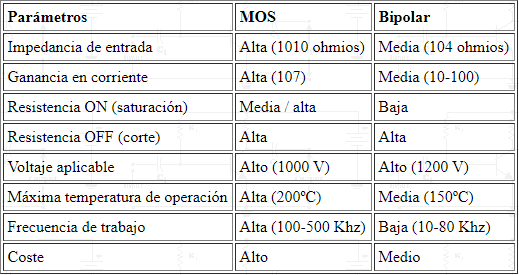
\includegraphics[scale=1]{Matriz.PNG} 
\end{figure}
Una limitación importante de todos los dispositivos de potencia y concretamente de los transistores bipolares, es que el paso de bloqueo a conducción y viceversa no se hace instantáneamente, sino que siempre hay un retardo (ton , toff). Las causas fundamentales de estos retardos son las capacidades asociadas a las uniones colector - base y base - emisor y los tiempos de difusión y recombinación de los portadores.
\subsection{Principios basicos de funcionamiento}
La diferencia entre un transistor bipolar y un transistor unipolar o FET es el modo de actuación sobre el terminal de control. En el transistor bipolar hay que inyectar una corriente de base para regular la corriente de colector, mientras que en el FET el control se hace mediante la aplicación de una tensión entre puerta y fuente. Esta diferencia vienen determinada por la estructura interna de ambos dispositivos, que son substancialmente distintas.

Es una característica común, sin embargo, el hecho de que la potencia que consume el terminal de control (base o puerta) es siempre más pequeña que la potencia manejada en los otros dos terminales.

En resumen, destacamos tres cosas fundamentales:

En un transistor bipolar IB controla la magnitud de IC.
En un FET, la tensión VGS controla la corriente ID.
En ambos casos, con una potencia pequeña puede controlarse otra bastante mayor.
Cuando el transistor está en saturación o en corte las pérdidas son despreciables. Pero si tenemos en cuenta los efectos de retardo de conmutación, al cambiar de un estado a otro se produce un pico de potencia disipada, ya que en esos instantes el producto IC x VCE va a tener un valor apreciable, por lo que la potencia media de pérdidas en el transistor va a ser mayor. Estas pérdidas aumentan con la frecuencia de trabajo, debido a que al aumentar ésta, también lo hace el número de veces que se produce el paso de un estado a otro.
Podremos distinguir entre tiempo de excitación o encendido (ton) y tiempo de apagado (toff). A su vez, cada uno de estos tiempos se puede dividir en otros dos.

Tiempo de retardo (Delay Time, td): Es el tiempo que transcurre desde el instante en que se aplica la señal de entrada en el dispositivo conmutador, hasta que la señal de salida alcanza el 10 de su valor final.

Tiempo de subida (Rise time, tr): Tiempo que emplea la señal de salida en evolucionar entre el 10 y el 90 de su valor final.

Tiempo de almacenamiento (Storage time, ts): Tiempo que transcurre desde que se quita la excitación de entrada y el instante en que la señal de salida baja al 90 de su valor final.

Tiempo de caída (Fall time, tf): Tiempo que emplea la señal de salida en evolucionar entre el 90 y el 10 de su valor final.

Por tanto, se pueden definir las siguientes relaciones :
\begin{equation}
Ton= td+tr
\end{equation}
\begin{equation}
Toff= ts+tg
\end{equation}
\begin{figure}[h!]
\centering
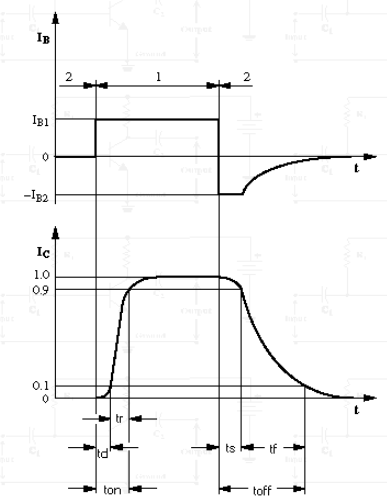
\includegraphics[scale=1]{Captura10.PNG}  
\end{figure}
Es de hacer notar el hecho de que el tiempo de apagado (toff) será siempre mayor que el tiempo de encendido (ton).
Los tiempos de encendido (ton) y apagado (toff) limitan la frecuencia máxima a la cual puede conmutar el transistor:
\begin{equation}
Fmax= \frac{1}{Fon + Foff}
\end{equation}
\subsection{Otros parametros importantes}
Corriente media: es el valor medio de la corriente que puede circular por un terminal (ej. ICAV, corriente media por el colector).
Corriente máxima: es la máxima corriente admisible de colector (ICM) o de drenador (IDM). Con este valor se determina la máxima disipación de potencia del dispositivo.

VCBO: tensión entre los terminales colector y base cuando el emisor está en circuito abierto.
VEBO: tensión entre los terminales emisor y base con el colector en circuito abierto.

Tensión máxima: es la máxima tensión aplicable entre dos terminales del dispositivo (colector y emisor con la base abierta en los bipolares, drenador y fuente en los FET).

Estado de saturación: queda determinado por una caída de tensión prácticamente constante. VCEsat entre colector y emisor en el bipolar y resistencia de conducción RDSon en el FET. Este valor, junto con el de corriente máxima, determina la potencia máxima de disipación en saturación.

Relación corriente de salida - control de entrada: hFE para el transistor bipolar (ganancia estática de corriente) y gds para el FET (transconductancia en directa).
\subsection{Modos de trabajo}
Existen cuatro condiciones de polarización posibles. Dependiendo del sentido o signo de los voltajes de polarización en cada una de las uniones del transistor pueden ser :
\begin{figure}[h!]
\centering
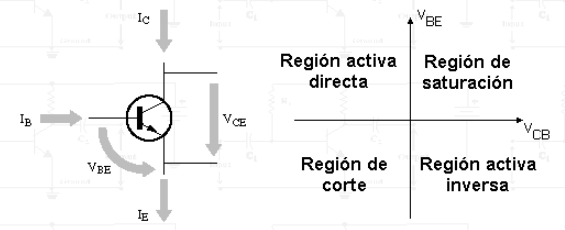
\includegraphics[scale=1]{Modos de trabajo.png}  
\end{figure}
Región activa directa: Corresponde a una polarización directa de la unión emisor - base y a una polarización inversa de la unión colector - base. Esta es la región de operación normal del transistor para amplificación.
 

Región activa inversa: Corresponde a una polarización inversa de la unión emisor - base y a una polarización directa de la unión colector - base. Esta región es usada raramente.
 

Región de corte: Corresponde a una polarización inversa de ambas uniones. La operación en ésta región corresponde a aplicaciones de conmutación en el modo apagado, pues el transistor actúa como un interruptor abierto (IC 0).
 

Región de saturación: Corresponde a una polarización directa de ambas uniones. La operación en esta región corresponde a aplicaciones de conmutación en el modo encendido, pues el transistor actúa como un interruptor cerrado (VCE 0).

Ecuación recta de carga para Ic: Vcc = Vce + (Ic x Rc)

Ecuación recta de carga para Ie  : Vcc = Vbe + (Re x Ie)

El transistor en base-emisor de comporta como un diodo, por eso la tensión base-emisor suele estar próxima a 0.7V

Ic = B x Ib
Ib = (Vcc - 0.7) / Rb
\end{document}